%%%%%%%%%%%%%%%%%%%%%%%%%%%%%%%%%%%%%%%%%%%%%%%%%%%%%%%%%%%%%%%%%%%%%%%%%%
%%%%%                         CHAPITRE 4                            %%%%%%
%%%%%%%%%%%%%%%%%%%%%%%%%%%%%%%%%%%%%%%%%%%%%%%%%%%%%%%%%%%%%%%%%%%%%%%%%%

\lhead[\fancyplain{}{\leftmark}]%Pour les pages paires \bfseries
      {\fancyplain{}{}} %Pour les pages impaires
\chead[\fancyplain{}{}]%
      {\fancyplain{}{}}
\rhead[\fancyplain{}{}]%Pour les pages paires 
      {\fancyplain{}{\rightmark}}%Pour les pages impaires \bfseries
\lfoot[\fancyplain{}{}]%
      {\fancyplain{}{}}
\cfoot[\fancyplain{}{\thepage}]%\bfseries
      {\fancyplain{}{\thepage}} %\bfseries
\rfoot[\fancyplain{}{}]%
     {\fancyplain{}{\scriptsize}}


%%%%%%%%%%%%%%%%%%%%%%%%%%%%%%%%%%%%%%%%%%%%%%%%%%%%%%%%%%%%%%%%%%%%%%%%%%
%%%%%                      Start part here                          %%%%%%
%%%%%%%%%%%%%%%%%%%%%%%%%%%%%%%%%%%%%%%%%%%%%%%%%%%%%%%%%%%%%%%%%%%%%%%%%%

\chapter{Robustness assessment}
\label{ch:4}

%==============================================================================	Résumé du chapitre

\begin{center}
\rule{0.7\linewidth}{.5pt}
\begin{minipage}{0.7\linewidth}
\smallskip

\textit{A markerless motion capture method is satisfying if it is accurate, fast, and robust. Robustness is deemed good when results are unchanged while adding constraints on the subject or on the environment. We challenge our workflow on walking, running, and cycling tasks, by adding people in the background, and by simulating challenging conditions: (Im) alters image quality (11-pixel Gaussian blur and 0.5 gamma compression); (4c) uses fewer cameras (4 vs. 8) which leads to unsolved occlusions; and (Cal) introduces calibration errors (1 cm vs. perfect calibration).\newline \newline
When averaged over all joint angles, stride-to-stride standard deviations lay between 1.7° and 3.2° for all conditions and tasks, and mean absolute errors (compared to the reference condition—Ref) ranged between 0.35° and 1.6°. For walking, errors in the sagittal plane were: 1.5°, 0.90°, 0.19° for (Im), (4c), and (Cal), respectively. As a consequence, Pose2Sim is robust enough for the 3D joint angle analysis of walking, running, and cycling, under challenging conditions. \newline\newline
This chapter is adapted from the article published in the Sensors: "Pose2Sim: An End-to-End Workflow for 3D Markerless Sports Kinematics—Part 1: Robustness" \cite{Pagnon2021}.
}


%\smallskip
\end{minipage}
\smallskip
\rule{0.7\linewidth}{.5pt}
\end{center}

\minitoc
\newpage


\section{Introduction}
\subsection{Robustness definition}

According to the review of \cite{Desmarais2021}, the performance of a method can be ranked regarding its accuracy, speed, or robustness. Accuracy is mostly assessed with MPJPE (Mean Per Joint Position Error); speed is evaluated either regarding computing complexity, or framerate when possible; and robustness is gauged through differences in the results while changing the system parameters only. \cite{Desmarais2021} points out that authors usually only consider accuracy, sometimes speed, but rarely robustness. However, robustness is of paramount importance in the context of sports, especially "in the wild". This chapter will focus on robustness, the next one on \nameref{ch:5}, and we will not focus on speed in this thesis (although chapter 3.4.5 broaches \hyperref[subsec:realtime]{Real time considerations}).

\cite{Moeslund2001} proposed to express robustness as the number of constraints on the subject or on the environment required for a motion capture system to be operational. Some of the assumptions they proposed have already been universally overcome by deep-learning-based methods. For example, no markers are involved anymore, the subject can wear their usual clothes (including loose pants or dresses \cite{Viswakumar2019}), and the background does not need to be static or uniform. Some other items remain an open problem.

For instance, most 3D methods assume that only one person lies in the camera field of view. This is a strong assumption, especially outdoors where people and athletes pass by and an operator is often present. Although it is starting to be addressed, standard solutions are yet to be determined \cite{Slembrouck2020,Bridgeman2019, Chu2021, Dong2019}. 

Other open questions lie in the environment, much less controlled in a sports context than in a lab, which can result in bad image qualities. \cite{Viswakumar2019} experienced that OpenPose is very robust to extreme lightning conditions. However, research has shown that pose estimations models are more robust to noise or brightness changes, while less robust to motion or to defocus blur \cite{Wang2021b}. And yet, in sports, the movement is not usually slow, continuous, nor limited to the sagittal plane.

Occlusions are, for the most part, solved by using a network of calibrated cameras. Since triangulation is computed using a least square method, a large amount of cameras will also blunt imprecision on the 2D joint estimations. \cite{Bala2020} showed that once correctly trained for 3D macaque pose estimation, eight cameras were enough to correctly infer 80\% of the 13 considered keypoints, while four cameras decreased the performance to about 50\%. However, a correct estimation of extremities such as feet and hands required more than eight cameras.

Camera calibration can be challenging outside, due to large volume spaces, bright light, and contrasting shades. As a consequence, it is close to impossible with the classic approach based on predefined objects with markers. Moreover, simple calibration with a checkerboard may cause errors on intrinsic and extrinsic camera parameters estimation \cite{Sun2005}. A calibration is generally considered acceptable if the average residuals of each camera (i.e., the root mean square error of the reprojection of the 3D reconstructed coordinates on the 2D image plane) is below 1 pixel. In metric terms, the markers-based Qualisys Track Manager software recommends redoing a calibration when the average residuals exceed 3 millimeters \cite{QTM2018}. The pinhole camera model gives an equivalence between pixel values on the image plane, and metric values on the object plane at the center of the scene, as demonstrated by Figure~\ref{fig_pixmeterscorrespondance} and Equation~\ref{eqn:errobjimg}. See Chapter 2.2.1 on \nameref{subsec:Pinhole model} or \cite{Dawson-Howe1994} for in-depth explanations.

\begin{figure}[!ht]
	\centering
	\def\svgwidth{1\columnwidth}
	\fontsize{10pt}{10pt}\selectfont
	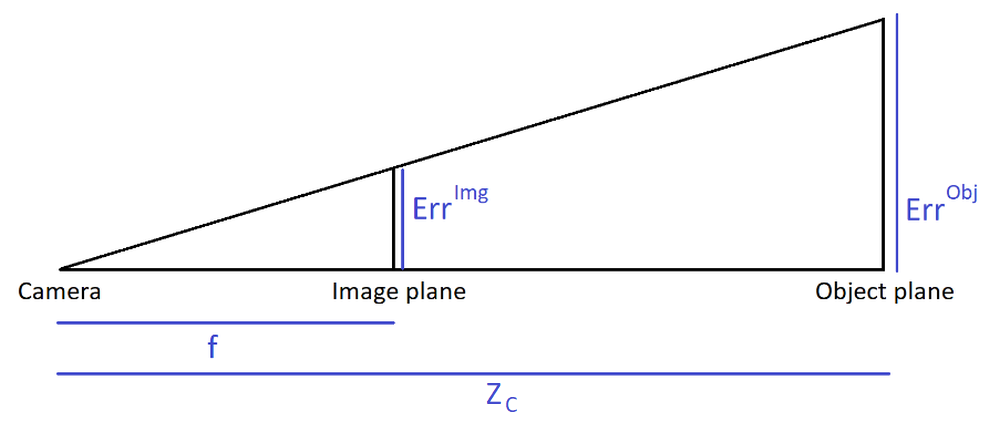
\includegraphics[width=\linewidth]{"../Chap4/Figures/Fig_PixelMeterCorrespondance.png"}
	\caption{The pinhole camera model permits a correspondence between image coordinates and object coordinates. f: focal distance, D: object to camera distance, $Err^{Img}$: error on image plane, $Err^{Obj}$: error on object plane. f and $Err^{Img}$ are usually expressed in pixels, while D and $Err^{Obj}$ are expressed in meters.}
	\label{fig_pixmeterscorrespondance}
\end{figure}

\begin{equation}
      Err^{Img} = \frac{f \times Err^{Obj}}{D} 
      \label{eqn:errobjimg}
\end{equation}


\subsection{Assessing robustness}

Before assessing the robustness of the workflow on walking, running, and cycling sequences, the relevance of the computed 3D full-body angles needs to be estimated. This will be done by comparing our angle results to those of a normative walking database. Further concurrent validation of the accuracy will be determined in the next chapter on \nameref{ch:5}. Repeatability will be evaluated by comparing movement cycles to each other, within each task and each capture condition. 

Robustness itself will be assessed through all three types of movements, in accordance with the open problems previously described:
\begin{enumerate}[itemsep=0em, topsep=0em, leftmargin=*]
      \item In addition to the person of interest, some people will be present in the background. 
      \item Image quality will be altered, by simulating a dark scene captured with defocused cameras objectives.
      \item Occlusions will become more challenging as we decrease the number of cameras. Moreover, cycling sequences will lead to more occlusions than walking or running ones.
      \item Calibration errors will be introduced by corrupting the calibration files.
\end{enumerate}

The underlying idea presented in this article is to verify whether modifying external environment parameters significantly impacts variability in joint angle estimation.


\section{Methods}
\subsection{Experimental setup}

To guarantee a tight control of the environment parameters, we captured our data in a dedicated studio platform called Kinovis \cite{Tsiminaki2014}, from which we were able to create realistic virtual views similar to outdoor video. This platform is a \(10 m \times 10 m \times 5.6 m\) green room equipped with 68 video cameras recording at 30 fps in 4 Mpixels resolution, for a practical acquisition space of about \(5 m  \times 5 m  \times 3 m\). The system computes 3D textured meshes by convex visual hull reconstruction \cite{Laurentini1994}. The meshes were inserted in a virtual environment composed of an environment texture map captured from a BMX racetrack, and a custom-made virtual floor. It should be noted that three people were present in the background, which introduced a realistic artifact of multiple subjects.

We developed a script for Autodesk Maya \cite{Maya1998} (see \nameref{subsec:viztools}) that allows us to render the textured mesh files, as well as to virtually set any cameras with specific properties (position, orientation, resolution, focal length, distortion, pixel size, binning factor). Views seen through virtual cameras can be saved as video files and visualized into a global 3D environment (Figure 3). The generated video files were used as input to the 3D kinematics pipeline.

For the purpose of this study, we created 8 virtual video cameras. Resolution was set to \(1280 \times 768\) pixels, focal length to 9 mm, pixel size to 5.54 µm, and no distortion nor binning was introduced. Binning refers to the process of grouping pixels in order to increase sensitivity to light, at the expense of decreasing resolution. Cameras were regularly distributed 8 m away from the center of the captured volume, at a height of 1 m, so that the whole body could be detected for a maximum of movement cycles. We then rendered the scene as video files from our virtual cameras and saved the exact calibration parameters. We applied a \(3 \times 3\) pixel Gaussian blur afterwards to reduce sharp edges of the virtual scene compositing (Figure~\ref{fig_smooth}). This resulting image quality was considered as “standard”.

\begin{figure}[!ht]
	\centering
	\def\svgwidth{1\columnwidth}
	\fontsize{10pt}{10pt}\selectfont
	\includegraphics[width=\linewidth]{"../Chap4/Figures/Fig_Smooth.png"}
	\caption{To smooth out sharp edges due to compositing, we applied a \(3 \times 3\) pixel Gaussian blur to the videos filmed from our virtual scene.}
	\label{fig_smooth}
\end{figure}


\subsection{Participant and protocol}

One healthy adult male subject (1.89 m, 69 kg) participated in the study. He provided his informed written consent prior to participating. The study was conducted in accordance with the Declaration of Helsinki \cite{Holm2013}. No requirement was given to him regarding his outfit. He was asked to perform three basic sports tasks: walking, running, and cycling. For all three tasks, the subject was given a moment beforehand to warm up and find a comfortable and regular pace, which he could then follow owing to the sound of a metronome:

\begin{itemize}[itemsep=0em, topsep=0em, leftmargin=*]
      \item \textit{Walking:} The subject walked in a straight line back and forth over the 10 m diagonal of the room. His body mesh could be fully reconstructed only in the central 5 m of the acquisition space, i.e., only roughly 2 gait cycles were acquired per walking line. His comfortable stride pace was 100 BPM (Beats per Minute). The stride length was not monitored. 
      \item \textit{Running:} The subject jogged in a straight line back and forth along the 10m diagonal of the room. His comfortable stride pace was 150 BPM (Beats per Minute). The stride length was not monitored.
      \item \textit{Cycling:} The subject cycled on a road bike placed on a home trainer. He himself adjusted the resistance and the height of the saddle prior to the capture. His comfortable cadence was 60 BPM.
\end{itemize}
As obtaining the textured meshes of the subject in the green Kinovis room involved filming simultaneously with 68 4 Mpixels cameras that generated a flow of over 8 gigabytes per second, the capture design limited the acquisition time to 45 s.


\subsection{Challenging robustness}

We challenged robustness with 3 challenging conditions, compared to a reference one.

\begin{itemize}[itemsep=0em, topsep=0em, leftmargin=*]
      \item \textit{Reference Condition (Ref):} The reference condition under which our 3D markerless kinematic system had to operate took advantage of the standard image quality, 8 available virtual cameras, and a perfect calibration. The standard quality corresponded to the unaltered images of the 3D scene filmed from our virtual cameras. The reference condition involved 8 virtual cameras, as a good compromise of what is feasible in real outdoor conditions. Moreover, a study on macaques showed that 8 cameras were enough to correctly infer 80\% of the 13 considered keypoints \cite{Bala2020}. The calibration could be considered perfect, since the virtual cameras were explicitly specified in the virtual environment.
      \item \textit{Poor Image Quality (Im):} Video quality was made blurrier and darker: a Gaussian blur (\(11 \times 11 px\)) was applied, as well as a 0.5 gamma compression (Figure~\ref{fig_imquality}). This simulated a dark scene captured with defocused camera objectives.
      \item \textit{Less Cameras (4c):} The 2D joint coordinates were triangulated with only 4 cameras, instead of 8 in the reference condition: one on each side, one in the front, and one in the back, set 90° apart from each other.
      \item \textit{Calibration Errors (Cal):} Calibration residuals are classically supposed to be under 1 px on the image plane or under 3 mm on the object plane. Using Equation~\ref{eqn:errobjimg} demonstrates that in our case 3 mm corresponds to 0.61 px. We chose to simulate a calibration error of 2 px, which corresponds to about 1 cm (Equation~\ref{eqn:errobjcal}).
      \begin{equation}
            Err^{Obj} = \frac{Err^{Img} \times D}{f} = \frac{2 \times 8}{\frac{9 \times 10^{-3}}{5.54 \times 10^{-6}}} = 9.8 \times 10^{-3} m
            \label{eqn:errobjcal}
      \end{equation} 
      The calibration error was simulated by translating the extrinsic parameters of each camera in a random direction. The norm was randomly picked in a normal distribution of mean 2 px and a standard deviation of 1 px. The mean of these 8 translations was ensured to be equal to \(2 ± 10^{-3}\) px.
\end{itemize}

\begin{figure}[!ht]
	\centering
	\def\svgwidth{1\columnwidth}
	\fontsize{10pt}{10pt}\selectfont
	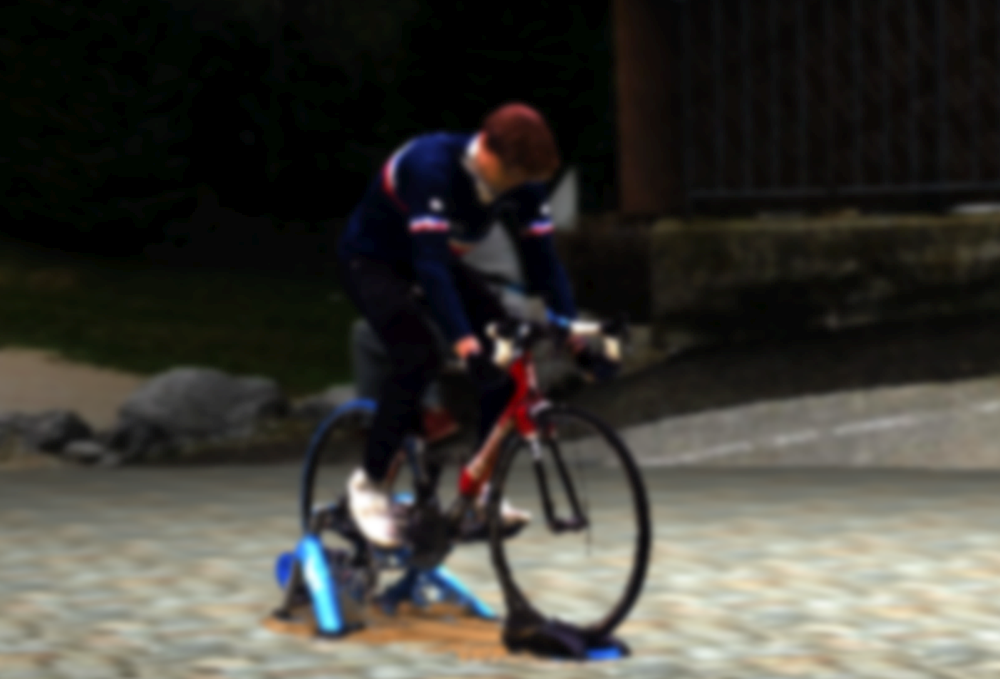
\includegraphics[width=\linewidth]{"../Chap4/Figures/Fig_ImQuality.png"}
	\caption{The image under poor image quality (Im) conditions. A Gaussian blur (\(11 \times 11 px\)) was applied, and a 0.5 gamma compression made the image darker.}
	\label{fig_imquality}
\end{figure}


\subsection{Markerless kinematics}

We applied OpenPose (version 1.6) on all the captured videos. We used the experimental body\_25b model (see~Figure\ref{fig_body25b}) with highest accuracy parameters, which is more accurate than the default body\_25 one and reduces the number of false positives \cite{Hidalgo2019}.

Then, we used Pose2Sim to robustly triangulate OpenPose outputs and feed the resulting 3D joint coordinates to OpenSim. The exact same parameters were used for all 4 conditions and all 3 movement tasks, in order to make sure the process did not induce any supplementary deviation to the compared results.




\subsection{Statistical analysis}
\blindtext


\section{Results}
\subsection{Data collection and 2D pose estimation}
\blindtext

\subsection{Pose2Sim tracking, triangulation, and filtering}
\blindtext

\subsection{Relevance, repeatability and robustness of angles Results}
\blindtext


\section{Discussion}
\subsection{Pose2Sim}
\blindtext

\subsection{Relevance, repeatability and robustness}
\blindtext

\subsection{Limits and perspectives}
\blindtext
